\documentclass[11pt]{beamer}
%\usetheme{CambridgeUS}
\usepackage[utf8]{inputenc}
\usepackage{amsmath}
\usepackage{amsfonts}
\usepackage{amssymb}
\usepackage{graphicx}
%\usepackage[outdir=./]{epstopdf}
\author{Hong Xiong}
%\title{}
%\setbeamercovered{transparent} 
\setbeamertemplate{navigation symbols}{} 
%\logo{} 
%\institute{} 
%\date{} 
%\subject{} 
\begin{document}

%\begin{frame}
%\tableofcontents
%\end{frame}

\begin{frame}
\includegraphics[width=\textwidth]{outdoor_dis_vs_RSSI_5_spot.eps} 
\end{frame}

\begin{frame}
\frametitle{Three mapping methods}
\begin{itemize}
\item rssi distance direct mapping
\item rssi distance fitting
\item rssi distance weighted fitting
\end{itemize}
\end{frame}

\begin{frame}
\includegraphics[width=\textwidth]{outdoor_RSSI_vs_dis.eps} 
\end{frame}


\begin{frame}
\includegraphics[width=\textwidth]{outdoor_rssi_dis_fit.eps} 
\end{frame}


\begin{frame}
\includegraphics[width=\textwidth]{outdoor_rssi_dis_fit_weighted.eps} 
\end{frame}

\begin{frame}
\includegraphics[width=\textwidth]{outdoor_rssi_dis_weighted_std_fitting.eps} 
\end{frame}

\begin{frame}
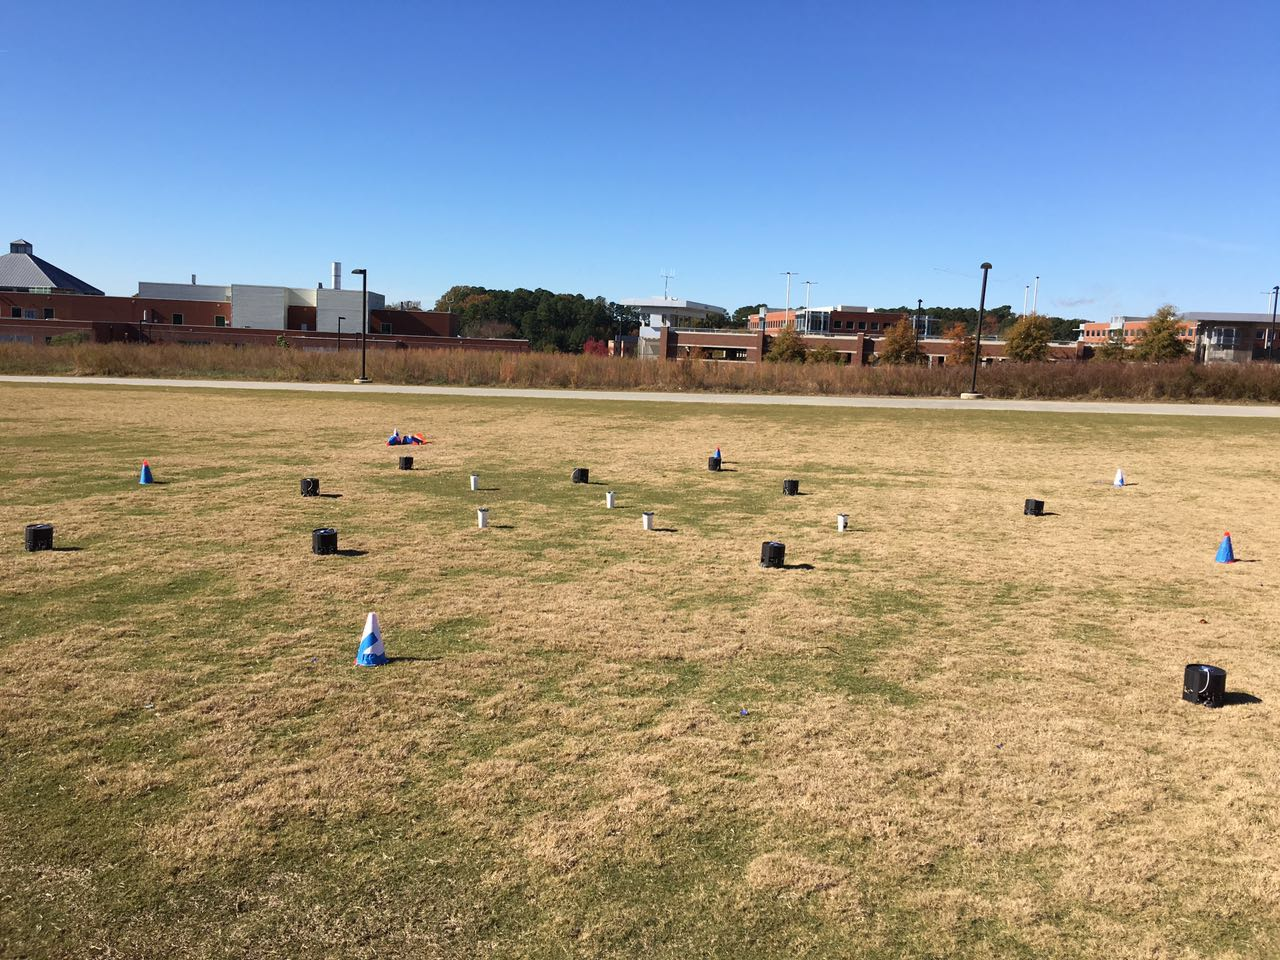
\includegraphics[width=\textwidth]{grass_wolfbot_setup.jpg} 
\end{frame}

\begin{frame}
\includegraphics[width=\textwidth]{grass_topo1.eps} 
\end{frame}

\begin{frame}
\frametitle{localization errors for kickloc}

\begin{tabular}{|c|c|c|c|}
\hline 
 & \multicolumn{3}{c|}{RSSI to Distance mapping model} \\ 
\hline 
Topology & direct  & fitting & weighted fitting \\ 
\hline
1 & 2.7585 & 2.3372 & 2.3672 \\
\hline
2 & 2.1123 & 2.1512 & 2.1573  \\
\hline
3 & 2.2952 & 2.2325 & 2.2487  \\
\hline
4 & 1.5604 & 1.4542 & 1.4762  \\
\hline
5 & 1.9285 & 1.8977 & 1.9164  \\
\hline
average & 2.1310 & 2.0146 & 2.0332  \\
\hline 
\end{tabular} 
\end{frame}

\begin{frame}
 \frametitle{localization result for topo4 method3}
\includegraphics[width=0.8\textwidth]{grass_final_mean_std_result_topo4_method3.eps} 
\end{frame}

\begin{frame}
 \frametitle{localization result for topo4 method3}
\includegraphics[width=\textwidth]{grass_final_mean_result_topo4_method3.eps} 
\end{frame}


\begin{frame}
\frametitle{average localization errors for different algorithms }
\begin{tabular}{|c|c|c|c|}
\hline 
 & \multicolumn{3}{c|}{RSSI to Distance mapping model} \\ 
\hline 
Algorithm & direct  & fitting & weighted fitting \\ 
\hline 
KickLoc & 2.1310 & 2.0146 & 2.0332 \\
\hline 
DV-distance & 2.7187 & 2.5311 & 2.5992  \\
\hline
Min-Max & 2.1845  &  2.0676  &  2.0704  \\
\hline
N-hop Lateration & 3.0825  &  2.8399  & 2.8816  \\
\hline
\end{tabular} 
\end{frame}


\end{document}
